\subsection{Data Model}
\subsubsection{Data Model and Back-end Structures}
\label{sec:datamodel}

With the overall requirements set we began working on the data model of the system with an initial focus on the database entities and relationships. The database entity-relationship model was sketched in LucidChart \footnote{Lucidchart is a web-based diagramming software which allows users to collaborate and work together in real time to create flowcharts, organisational charts, website wireframes, UML designs, mind maps, software prototypes, and many other diagram types.} using the notation from Database Management Systems \cite{dbbook}. The complete E-R model is shown in Figure ~\ref{fig:erd}.

\begin{figure}[t]
	\centering
	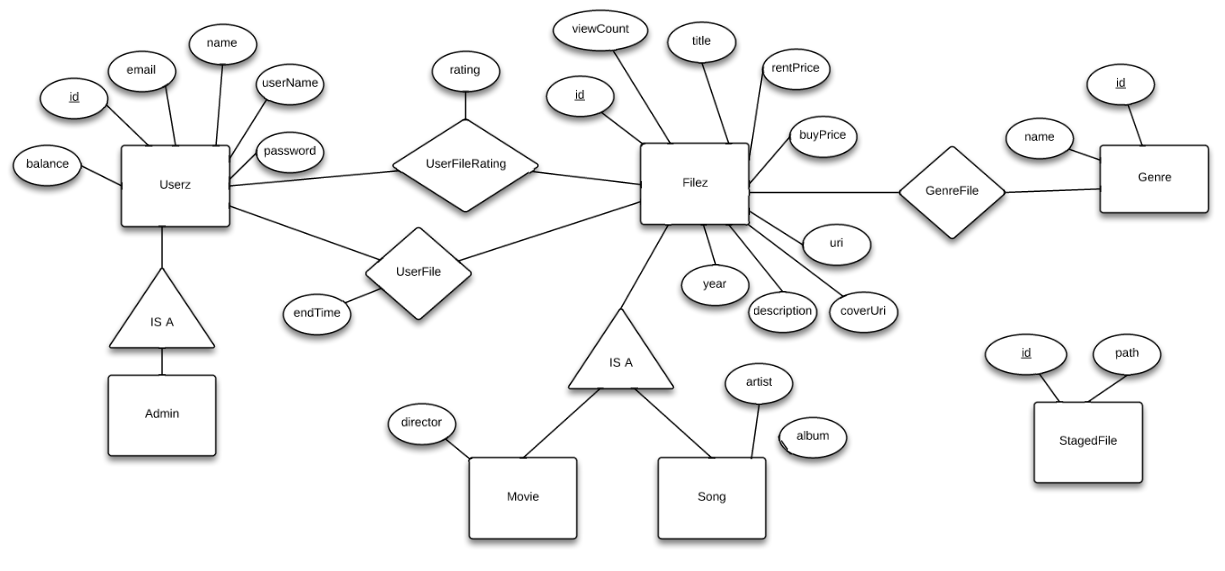
\includegraphics[scale=0.5]{./p1design/erdmodel.png}
	\caption{Our Entity Relationship Model}
	\label{fig:erd}
\end{figure}

Our E-R model follows a naming scheme, where each table is named after the real domain object it represents (singularized), with junction tables named by a concatenation of the tables linked. The naming scheme of junction tables are shown in Figure ~\ref{fig:junctionfigure}.


\begin{figure}[hbt]
	\centering
	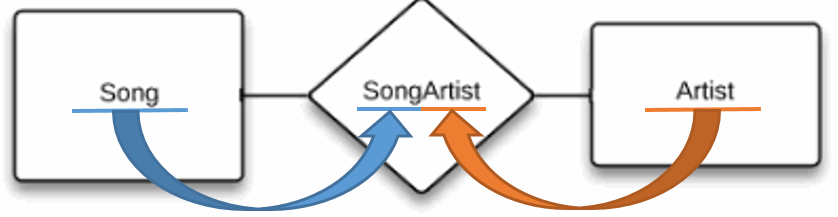
\includegraphics[scale=0.5]{./p1design/junctionfigure.png}
	\caption{Example of concatenated naming for junction tables.}
	\label{fig:junctionfigure}
\end{figure}


Where several junction tables exist between the same entities, we append an additional description string to the name (as seen in "UserFile\textit{Rating}").
Our decision to use the domain objects' names singularized caused problems with the “User” and “File” tables, since these names are reserved keywords in MS SQL. We updated said tables by appending a ‘s’ to the name (making it plural), but we kept the names singularized in the junction tables.

Besides creating a database structure capable of holding all the data needed for our use cases, we wanted to avoid redundant data. Our choice to avoid redundant data stems from the wish to eliminate anomalies within the database of which redundant data is a key cause. Anomalies are known to weaken the integrity of the database \cite{dbbook} due to irregular or inconsistent data, and we believe integrity is a key characteristic of a database dealing with users, their money, and their property. We enforced this constraint by applying a database normalization (third normal form) to our design, which is known to be free of update, insertion, and deletion anomalies.

\subsubsection{Designing for Extendability}
\label{sec:extendability}
During the design of our entity relationship model, we took time to brainstorm how the design might evolve during the lifespan of the product and how the datamodel might accommodate to those changes. We settled on two plausible cases
\begin{itemize}
\item A need for several types of medias
\item A need for several types of user roles
\end{itemize}
In the following we will explain how we designed for extendability in the context of the first case, but the principle applies to them both.
The naïve solution would be to create a new table for each media type e.g. 
\textbf{Song (id, title, artist, album, coverURI, rentPrice, …)} or
\textbf{Movie (id, title, director, coverURI, rentPrice, …)}
This will however create a lot of duplicate columns in different tables. If we wanted to add new information to our media types later, e.g. a “viewCount” (which did actually happen) this would need to be added to every media table.
The realization that several columns of information is shared across the media suggest for an inheritance based approach, where the shared columns are placed in a “super table”, while every media table will take part in an IS-A relationship with said “super table”. This is the design that can be seen in Figure ~\ref{fig:erd}.

With our minds set on centralizing the common media attributes in the Files super table, we noted that both a movie director and a song artist could be gathered under a common label "Creator". The Files table would then be connected to a "person" table, which would store both song artists and movie directors.
\begin{figure}[hbt]
	\centering
	\centerline{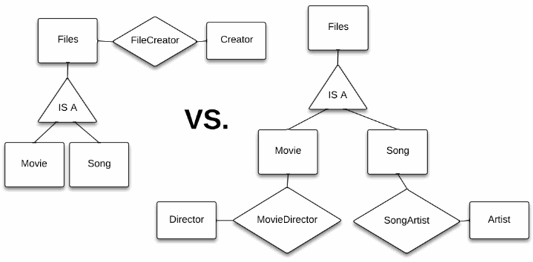
\includegraphics[scale=0.52]{./p1design/dilemma.png}}
	\caption{Example of the dilemma cases}
	\label{fig:erddilemma}
\end{figure}

We discussed this design and noted that it could not maintain the current constraint that only songs are linked to artists and only movies to directors. In addition we would not be able to extend the information on artists without extending it for directors too. This led to the decision to keep them seperate, although they are conceptually very close.

Later in the project we became aware that the above dilemma also applies to the concept of genres with the implication that a song could be linked to the genre "Horror", which does not make sense. As such the design of the genres-relation does not match our established design philosophies and we believe that this could (and should) be improved upon in any later revision of the project.

\subsubsection{Accessing the Database}
\label{sec:databaseaccess}
After having designed the database structure we had to decide how to access and utilize the database in the best suited way for our web service. We quickly settled for a C\#/WCF-based web service, since every group member had about the same experience in that platform from other ITU courses.
With access to the .NET framework, we considered to make use of the Entity Framework for our database interactions and general object-relational mapping. However several group members had been experiencing some inconvenient performance issues in previous projects. We do believe performance is an important aspect of our service and research has shown that users of the internet have become very impatient with regards to response times \cite{webusersflee}. We also deemed our queries and database interaction to be fairly simple, thus having no real need for most of the functionality in the Entity Framework. After a discussion it became clear that the only real benefit of using the framework was the possibility of faster prototyping. With our emphasis on a solid performance we choose to spend a little more time developing our own database access layer in order to maintain a more direct control over the performance of our solution.


\subsubsection{From Entities to Classes}
Although supporting declarative and functional features, C\# has been designed with the object oriented paradigm in mind \cite{csharpecma}, and as such we decided to use an object oriented approach for our back-end solution. 

We created several object oriented containers (classes) capable of holding the data of our web service. An example of our internal data classes capable of holding media can be seen in Figure ~\ref{fig:orm}.
\begin{figure}[hbt]
	\centering
	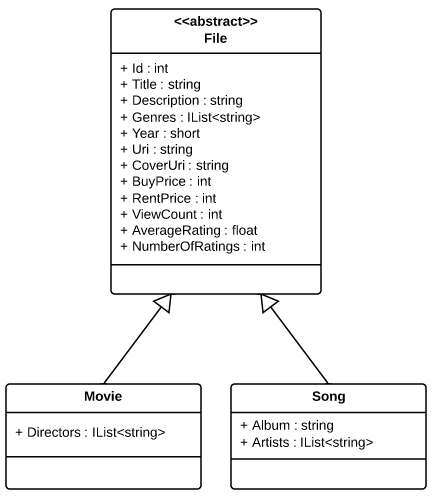
\includegraphics[scale=0.7]{./p1design/orm.png}
	\caption{Example of our oject oriented representation of the datamodel.}
	\label{fig:orm}
\end{figure}

This object oriented structure is derived from the IS-A relationship of the file concept in our database with general attributes (C\# properties) in the super class and unique attributes in the sub classes.

\subsubsection{Lazy loading}

Our objects are designed with \emph{lazy loading} in cases where a seperate database table is needed in order to set a property. Lazy loading is a design pattern, which defers the initialization of a variable until the variable is needed for the first time. This means that when an instance of the user class is prompted to answer if the user is an administrator/manager, the answer will be loaded and stored in the object for future reference. If the user object is never asked for the value of this property, then the value will never be retrieved from the database. In practice this looks like shown in Figure ~\ref{fig:lazyload}.

\begin{figure}[hbt]
	\centering
	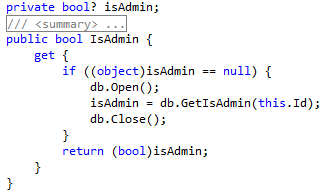
\includegraphics[scale=1]{./p1design/lazyload.png}
	\caption{Example of our use of lazy loading. A property from other tables is loaded when read for the first time.}
	\label{fig:lazyload}
\end{figure}


This design has potential to increase the performance of our solution in cases where, for instance, only the username of a user object is of interest, since no extra queries or joins with other database tables will be executed. In hindsight our design does not need this feature, as the lazy loaded properties are used extensively, thus causing several queries per object on the average. A solution with one query and joined tables might have been preferable, since the database would then not have to handshake, allocate connection buffers, etc. several times per object. As such, with regards to our use of lazy loading, we might have fell victim to "premature optimization" \cite{premoptim}, but we have no test measurements of the actual performance loss.


\subsubsection{Supported workflows}
Our datamodel supports all the workflows presented in our use cases, and it
does so by abstracting over the database design and relying on object oriented
container classes, which can be retrieved by a few calls to our database access
layer. An example use of the back-end is shown here in the context of the
following requirement:

\begin{itemize}
\item A user must be able to locate a specific movie/song through text search, matching movies with any property matching the text string.
\end{itemize}

Our back-end supports the above use case through only 4 lines as seen in Figure ~\ref{fig:moviesearch}.
\begin{figure}[hbt]
	\centering
	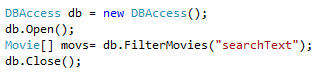
\includegraphics[scale=1]{./p1design/moviesearch.png}
	\caption{Example use of our back-end structure in the context of a use case.}
	\label{fig:moviesearch}
\end{figure}
